\documentclass{article}

\usepackage{listings} % for including MATLAB code
\usepackage{graphicx} % for including images
\usepackage{amsmath}

\title{80846 - Report - 4th}
\author{GU JUN, 6132230056-4}
\date{\today}

\begin{document}

\maketitle

\section*{Intruoduction}


This report is the 4th report of the course 80846. In this report, I will show the results of the three controllers:

Computed torque controller, Desired task space trajectory controller, and Adaptive controller.\\ 

The first controller is the Computed torque controller, which is a simple controller that can track a desired torque trajectory.

Based on this controller, with an inverse kinematics block, we can design a desired task space trajectory controller.

Or replacing $ M $ matrix with $\hat{M}$, which is updating with an adptive law, we can design a adptive controller.

\section{\centering \Large Computed torque controller}

\subsection*{Problem Statement}

According to the class, we are required to complete a controller that can track a torque function $q_d(t)$. 

I use the $sin$ function with $0.5 \pi$ shift on $y$.



% model of the system
\subsection{Simulink Model}
\begin{figure}[ht]
    \centering
    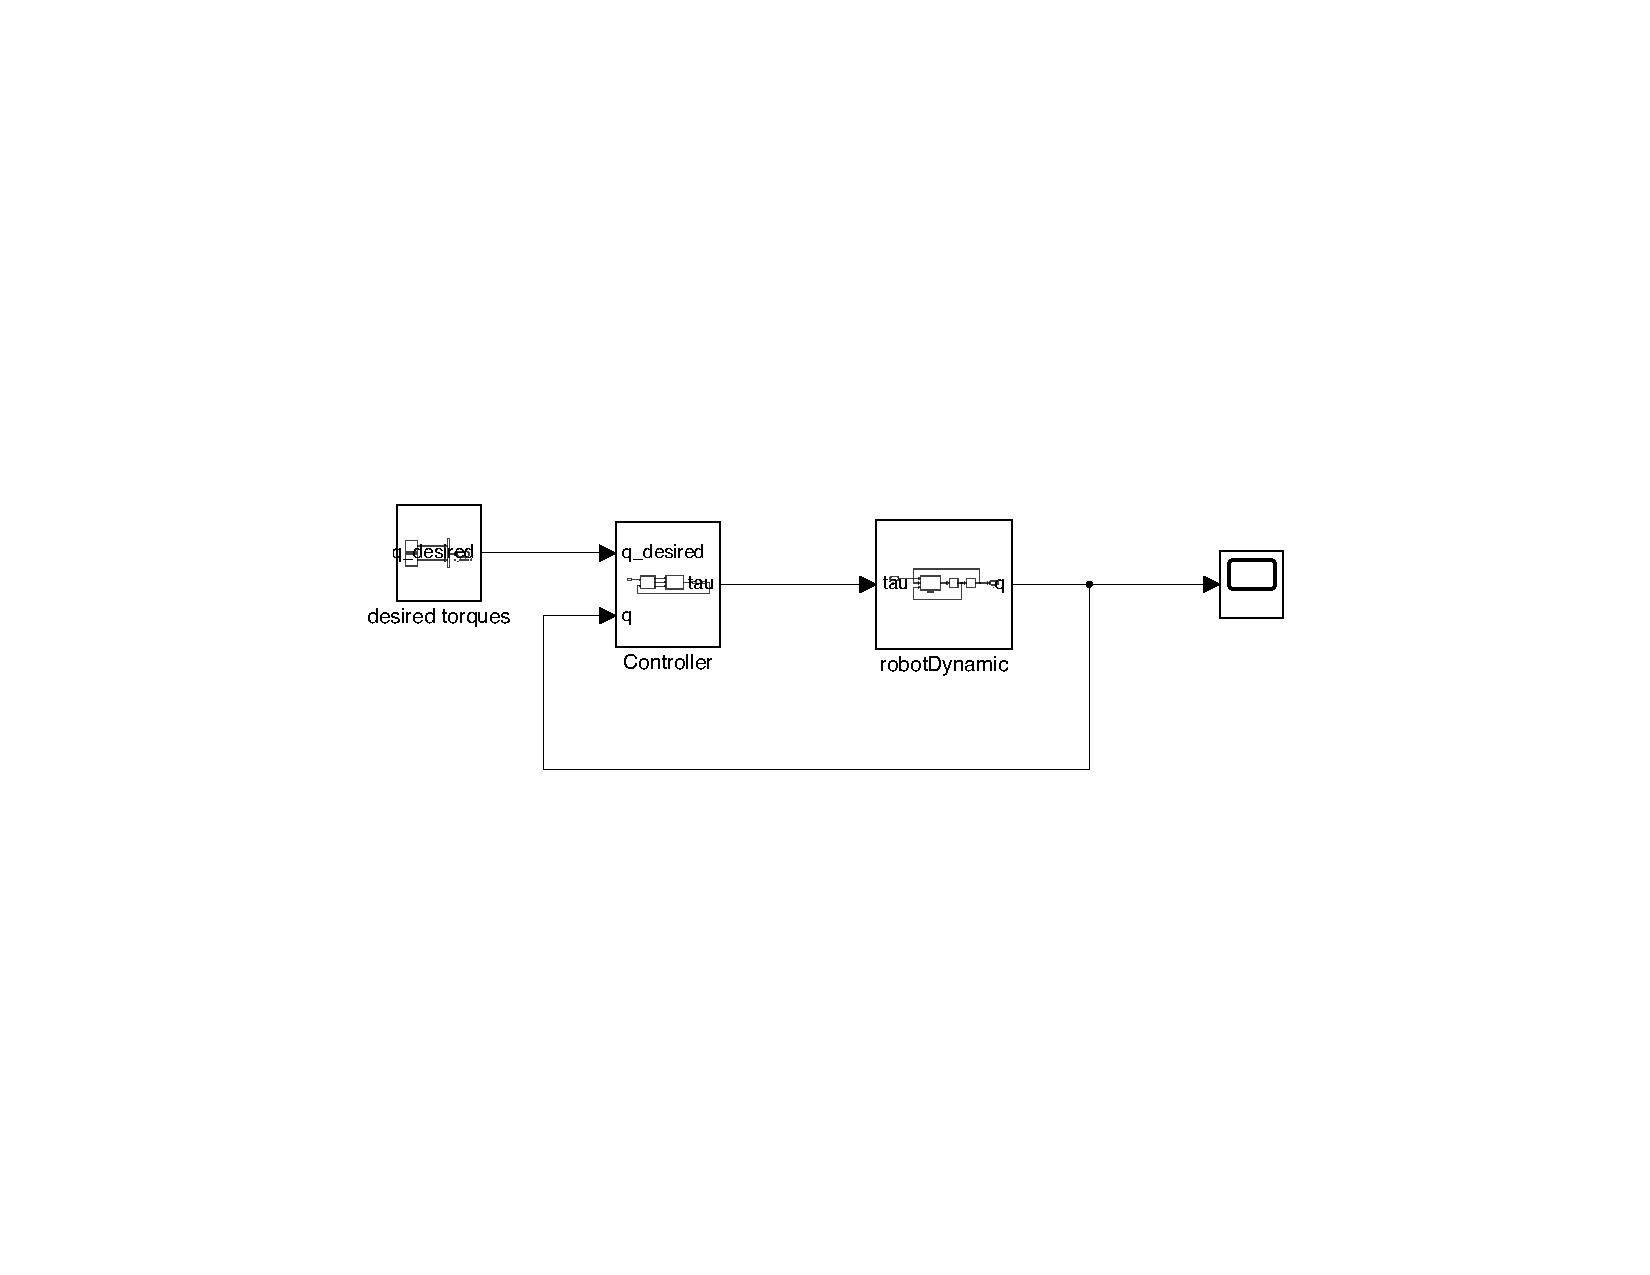
\includegraphics[width=0.9\textwidth]{figures/model_computed.pdf}
    \caption{Simulink Model of the system for the Computed torque controller}
    \label{fig:model_computed}
\end{figure}
See the Figure \ref{fig:model_computed}.

% formulas and source codes
\subsection{Formulas and Source Codes}
This part includes the formulas and source codes for the controller with the Jacobian matrix and forward kinematics blocks.
This part includes the formulas and source codes for the inverse dynamics
\subsection*{Inverse Dynamics}
According to the formula below, we need to calculate the $\tau_d$\\
    \begin{equation}
        \tau=\tau_d+k_p(q_d-q)+k_v(\dot{q}_d-\dot{q})
    \end{equation}
To calculate $\tau_d$, I use inverse dynamics.\\ 
\begin{equation}
    \tau_d = M \Ddot{q_d} + V \dot{q_d} + G
\end{equation}
Where $M$, $V$, $G$ have been mentioned in the past lectures.\\
The source code is shown below:
\begin{lstlisting}[language=Matlab, basicstyle=\small\ttfamily]


I1 = 0.05;
m1 = 1.5;
lg1 = 0.2;
lr1 = lg1 / 2;

I2 = 0.01;
m2 = 0.5;
lg2 = 0.2;
lr2 = lg2 / 2;

g = 9.8;

M = [m1 * lr1^2 + I1 + m2 * lg1^2, m2 * lg1 * lr2 * cos(q_desired(2));
        m2 * lg1 * lr2 * cos(q_desired(2)), m2 * lr2^2 + I2];

V = [-m2 * lg1 * lr2 * qd_desired(2)^2 * sin(q_desired(2));
    m2 * lg1 * lr2 * qd_desired(1)^2 * sin(q_desired(2))];

G = [m1 * g * lr1 * cos(q_desired(1)) + m2 * g * lg1 * cos(q_desired(1));
    m2 * g * lr2 * cos(q_desired(1) + q_desired(2));];

tau_d = M * qdd_desired + V + G;

    
\end{lstlisting}

\subsection*{Controller}
For the controller, there is just a little change.\\

The source code is shown below:\\

\begin{lstlisting}[language=Matlab, basicstyle=\small\ttfamily]

    function tau = controller(error, derror, tau_d)

    kp = [10, 0;
           0, 10];


    kd = [1, 0;
            0, 1];

    tau = kp * error + kd * derror + tau_d;
\end{lstlisting}


\subsection{Simulation Results}

\begin{figure}[ht]
    \centering
    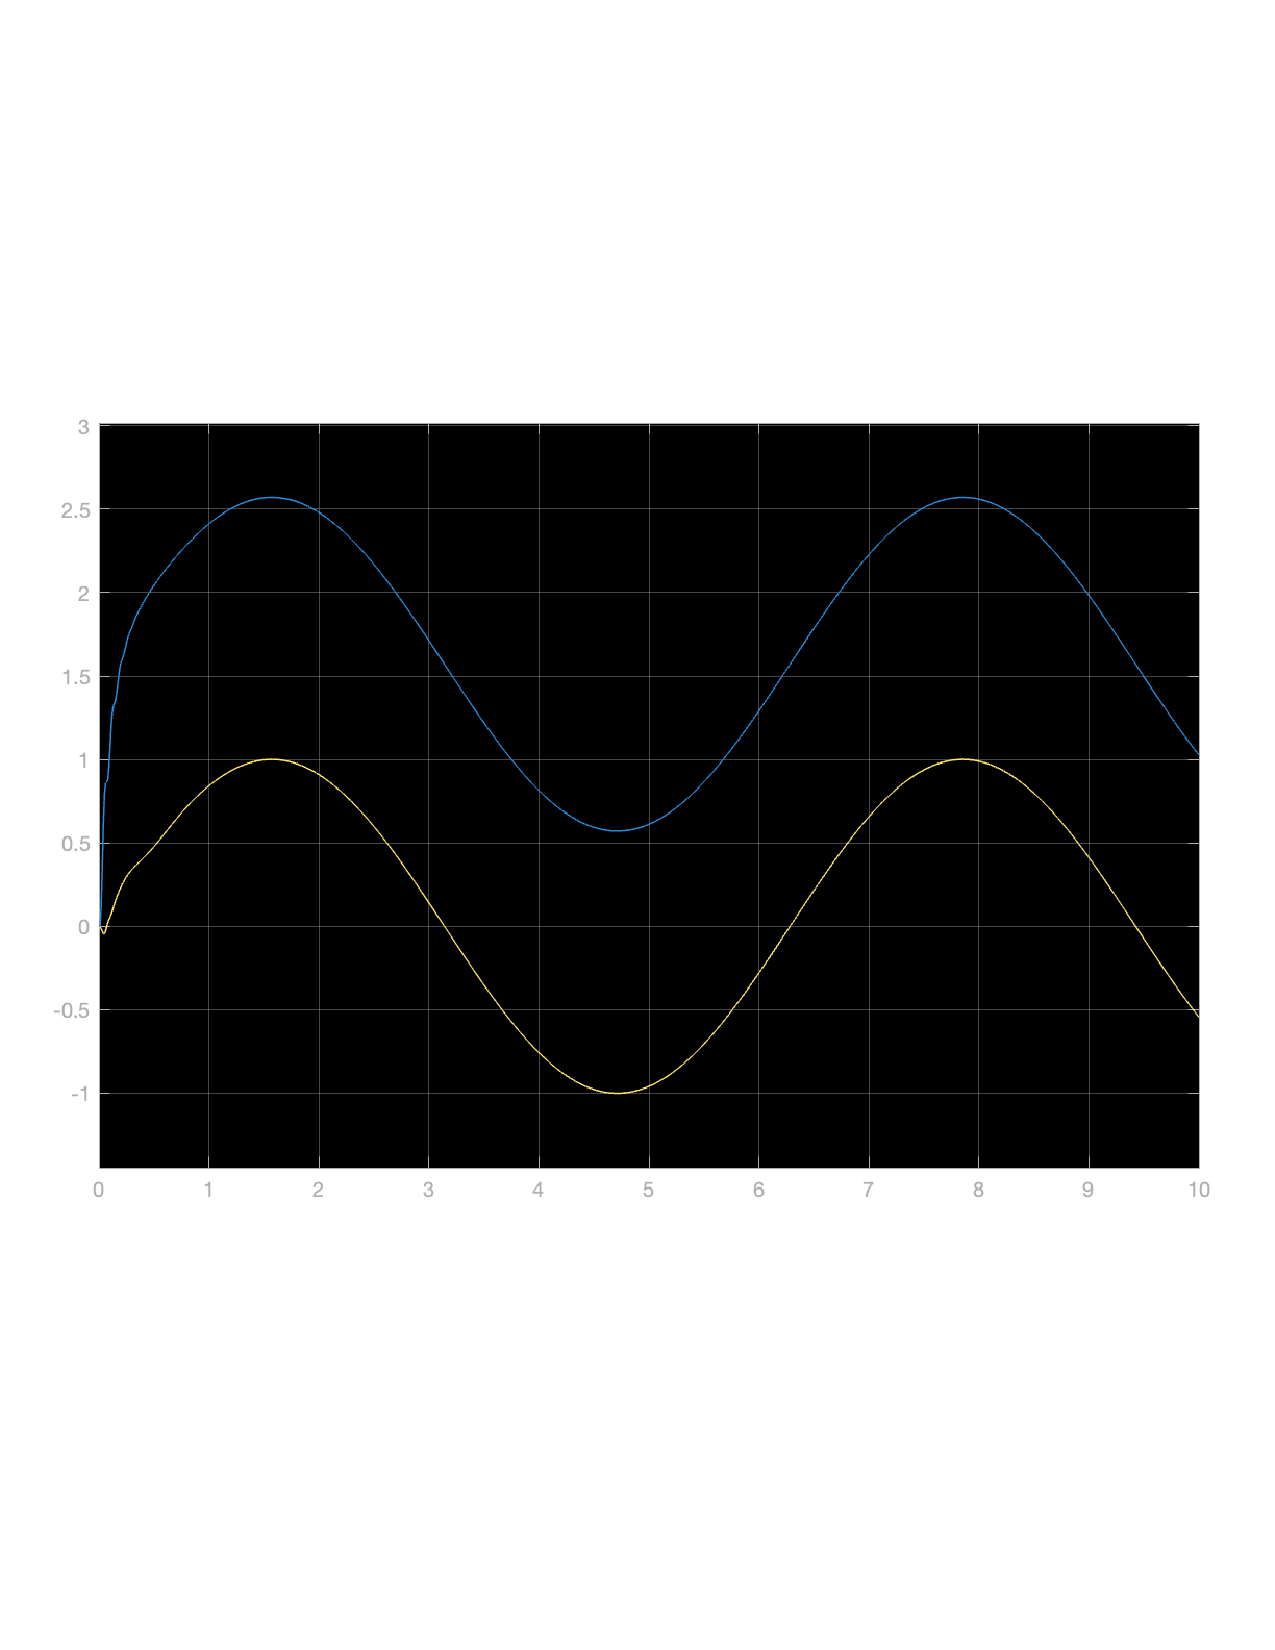
\includegraphics[width=0.8\textwidth]{figures/result_computed.pdf}
    \caption{Result Plot, error disappeared after 1 second}
    \label{fig:result_computed_plot}
\end{figure}

After some tuning of the gains, I got the following Figure \ref{fig:result_computed_plot}. \\





\newpage

\section{\centering \Large Desired task space trajectory controller} 

\subsection*{Problem Statement}

According to the class, we are required to complete a controller that can track a trajecoty in task space.\\

I use $x = 0.2 sin(t)$, $y = 0.2 cos(t)$ as the desired trajectory.\\

To do this, I need to calculate inverse kinematics for the robot, instead of using the Jacobian matrix, I directly calculate the inverse kinematics for this simple case.\\

The model of the system is the same as the Computed torque controller, so I will not show it again.\\ But I will show subsytem of the inverse kinematics block.\\

% model of the system
\subsection{Simulink Model}

See the Figure \ref{fig:model_ik} below.
\begin{figure}[ht]
    \centering
    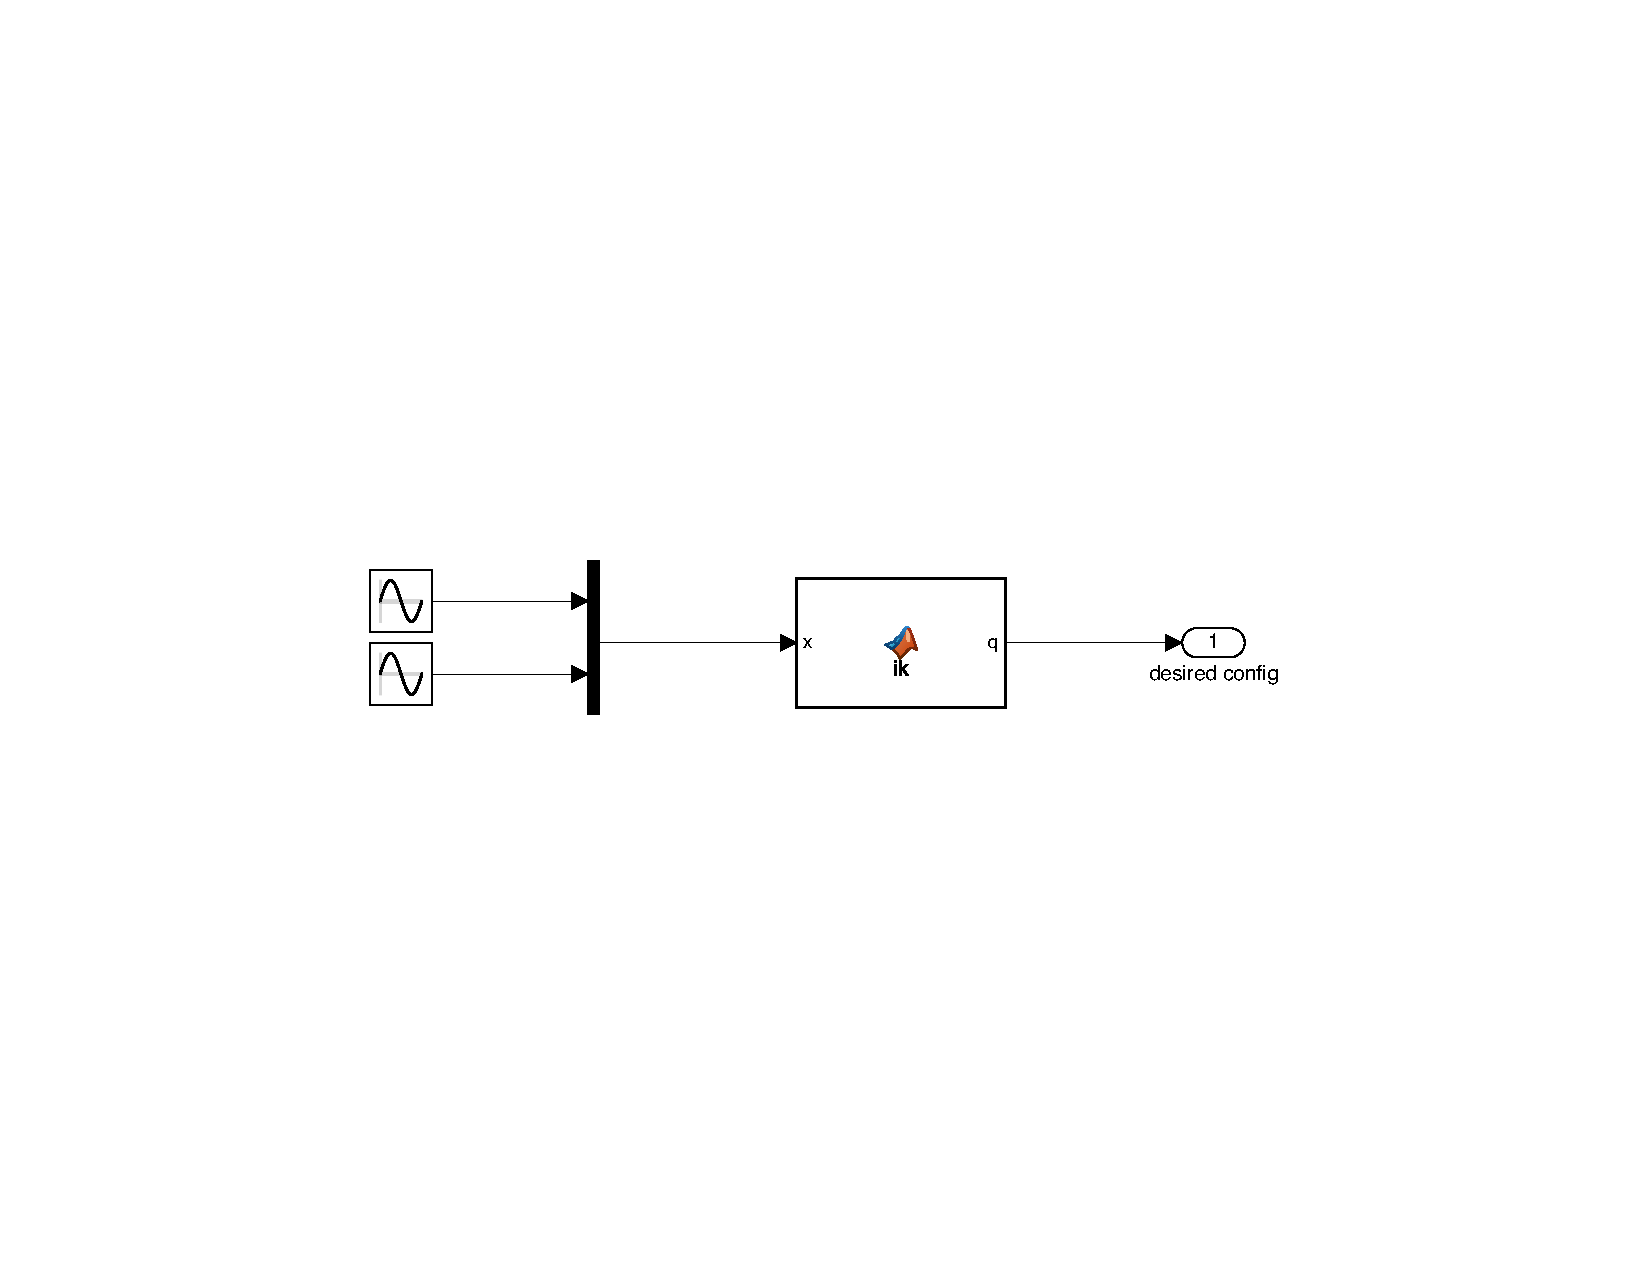
\includegraphics[width=0.9\textwidth]{figures/desiredTaskSpaceIKModel.pdf}
    \caption{Simulink Model of the subsystem for the how to calculate the desired joint angles}
    \label{fig:model_ik}
\end{figure}



% formulas and source codes
\subsection{Formulas and Source Codes}
This part includes the formulas and source codes for the inverse kinematics block.

\subsection*{Inverse Kinematics}
According to the formula below, we need to calculate the $\theta_2 $\\
\begin{equation}
    \cos \left(\theta_2\right)=\frac{x^2+y^2-L_1^2-L_2^2}{2 L_1 L_2} 
\end{equation}

\begin{equation}
    \theta_2=\arccos \left(\frac{x^2+y^2-L_1^2-L_2^2}{2 L_1 L_2}\right)
\end{equation}

To calculate the $\theta_1$, we can use the following formula:


\begin{equation}
    k 1=L_1+L_2 \cos \left(\theta_2\right) 
\end{equation}

\begin{equation}
    k 2=L_2 \sin \left(\theta_2\right) 
\end{equation}

\begin{equation}
    \theta_1=\arctan 2(y, x)-\arctan 2(k 2, k 1)
\end{equation}
    
The source code is shown below:
\begin{lstlisting}[language=Matlab, basicstyle=\small\ttfamily]

    function q = ik(x)
    L1 = 0.2;
    L2 = 0.2;


    d = sqrt(x(1)^2 + x(2)^2);
    
    if d > (L1 + L2) || d < abs(L1 - L2)
        error('The point is not reachable.');
    end
    
    cosTheta2 = (x(1)^2 + x(2)^2 - L1^2 - L2^2) / (2 * L1 * L2);
    theta2 = acos(cosTheta2);
    
    theta2_alt = -acos(cosTheta2);
    
    % Compute the intermediate values for theta1 calculation
    k1 = L1 + L2 * cos(theta2);
    k2 = L2 * sin(theta2);
    
    % Compute theta1
    theta1 = atan2(x(2), x(1)) - atan2(k2, k1);    
    
    k1_alt = L1 + L2 * cos(theta2_alt);
    k2_alt = L2 * sin(theta2_alt);
    


    q = [0; 0;];
    % Return the primary solution by default
    q(1) = theta1;
    q(2) = theta2;
end

    
\end{lstlisting}

\subsubsection*{Controller}
For the controller, there is no changes.\\


\subsection{Simulation Results}

After some tuning of the gains, I got the Figure \ref{fig:result_task_space_trajectory}. \\
\begin{figure}[ht]
    \centering
    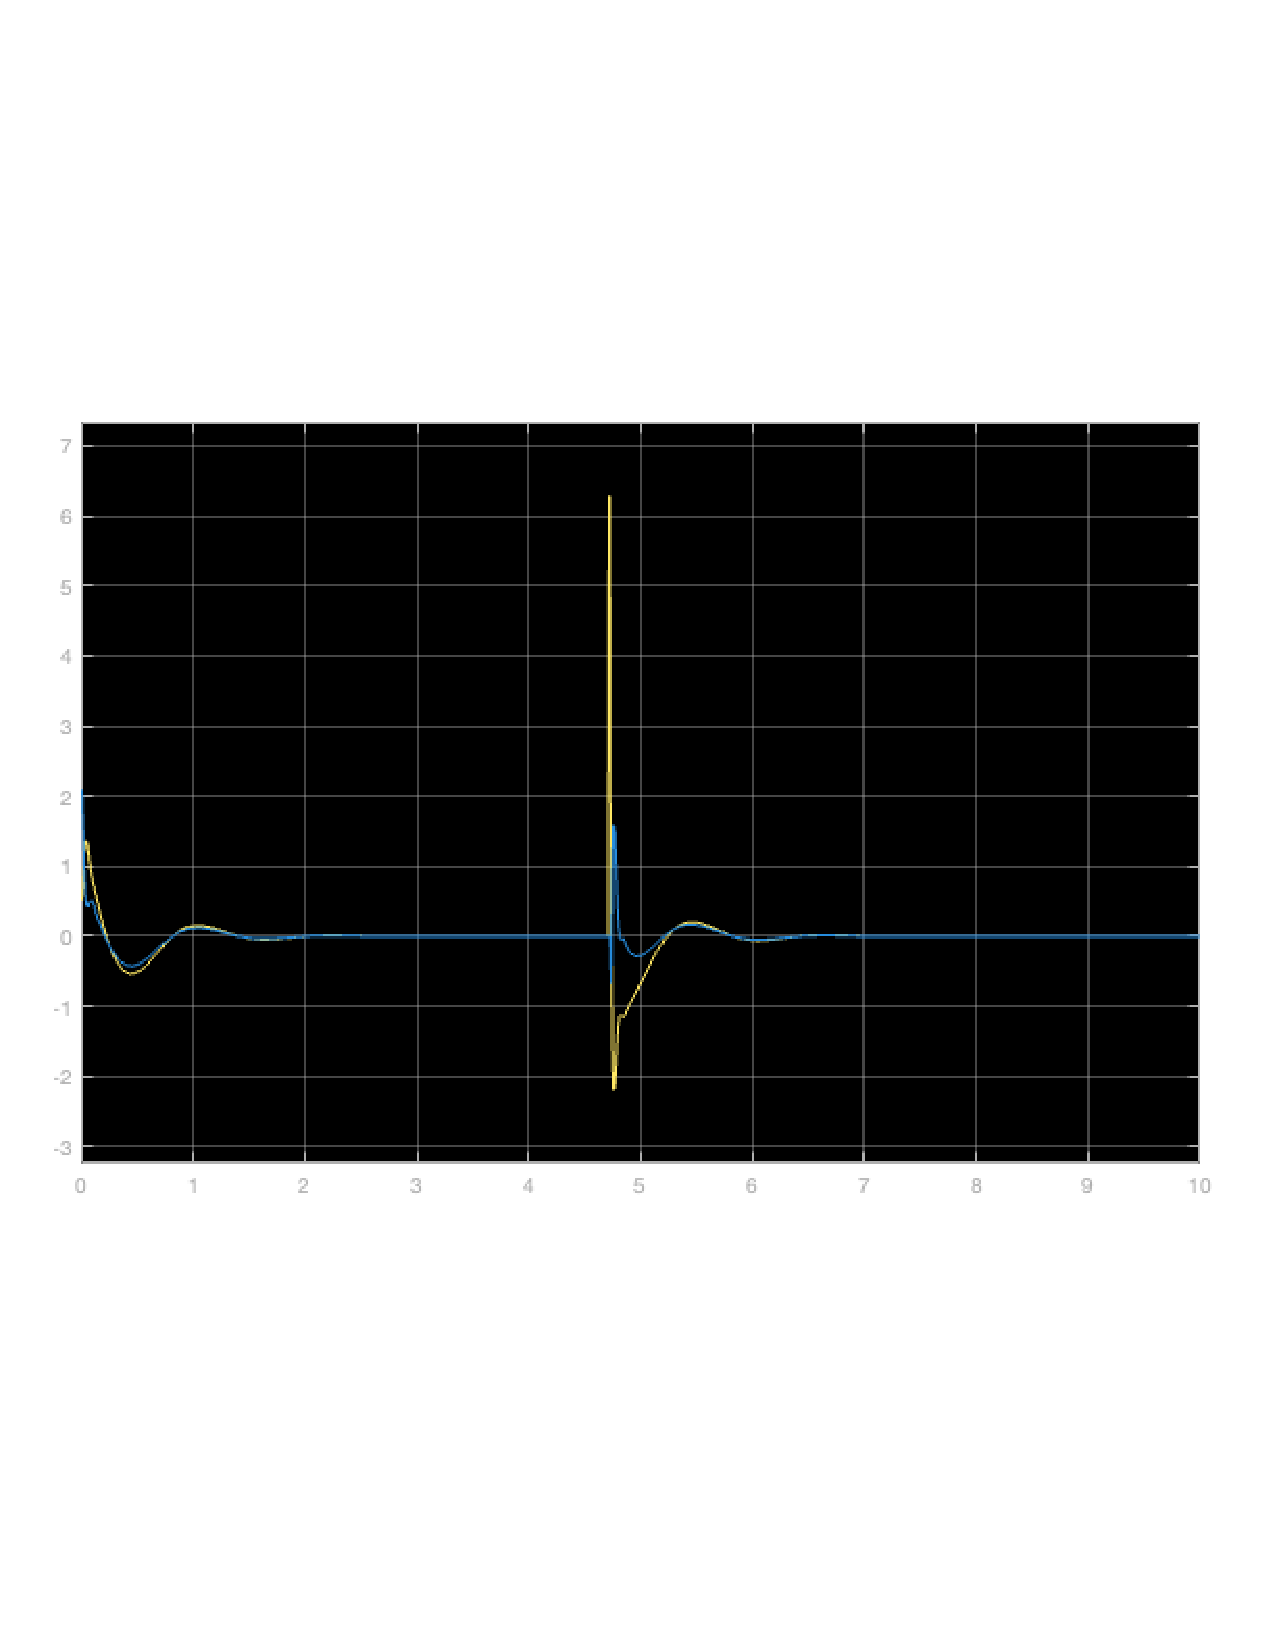
\includegraphics[width=0.8\textwidth]{figures/result_task_space_trajectory.pdf}
    \caption{Result Plot, there is a shake in the middle}
    \label{fig:result_task_space_trajectory}
\end{figure}




\newpage

\section{\centering \Large Adptive controller} 

\subsection*{Problem Statement}

We need to design a adaptive law block and use it to calculate the $\tau_d$\\

% model of the system
\subsection{Simulink Model}

I only show the inverse Dynamics part of the model.
See the Figure \ref{fig:model_inverseDynamics} below.
\begin{figure}[ht]
    \centering
    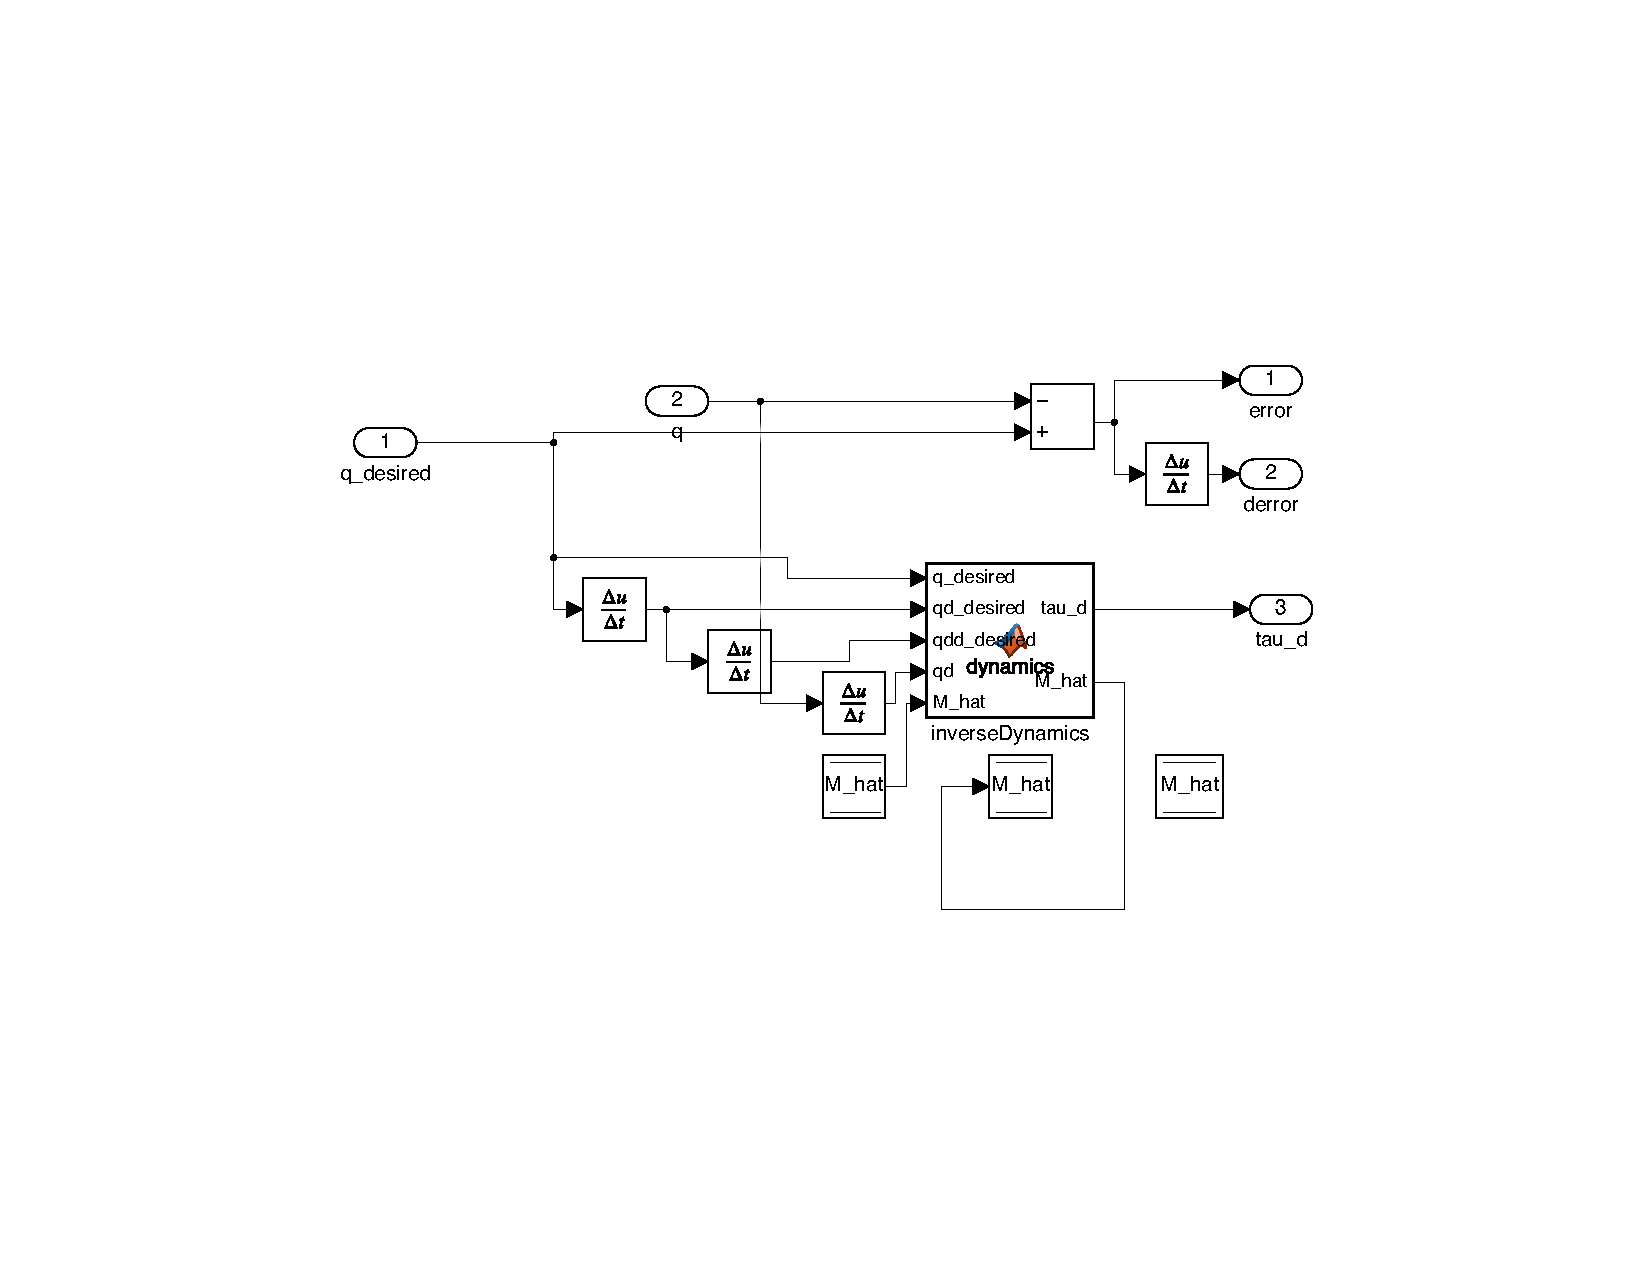
\includegraphics[width=0.9\textwidth]{figures/model_inverseDynamics.pdf}
    \caption{Simulink Model of the system for the Computed torque we needs}
    \label{fig:model_inverseDynamics}
\end{figure}

% formulas and source codes
\subsection{Formulas and Source Codes}
This part includes the formulas and source codes for the adaptive law
\subsection*{Inverse Dynamics}
    \begin{equation}
        \tau=\hat{M}(q) \ddot{q}_d+\hat{C}(q, \dot{q}) \dot{q}_d+\hat{G}(q)
    \end{equation}

For simple the question, I only apply the adaptive law to $\hat{M}$, other parameters are still calculated by old formula.\\

The source code is shown below:
\begin{lstlisting}[language=Matlab, basicstyle=\small\ttfamily]


    function [tau_d, M_hat]  = dynamics(q_desired, qd_desired, qdd_desired, qd, M_hat)


    I1 = 0.05;
    m1 = 1.5;
    lg1 = 0.2;
    lr1 = lg1 / 2;
    
    I2 = 0.01;
    m2 = 0.5;
    lg2 = 0.2;
    lr2 = lg2 / 2;
    
    gamma = 0.1;
    
    g = 9.8;
    
    M_hat = M_hat + gamma * (qdd_desired .* (qd_desired - qd));
    
    V = [-m2 * lg1 * lr2 * qd_desired(2)^2 * sin(q_desired(2));
        m2 * lg1 * lr2 * qd_desired(1)^2 * sin(q_desired(2))];
    
    G = [m1 * g * lr1 * cos(q_desired(1)) + m2 * g * lg1 * cos(q_desired(1));
        m2 * g * lr2 * cos(q_desired(1) + q_desired(2));];
    
    tau_d = M_hat * qdd_desired + V + G;
    
    end
    
\end{lstlisting}

\subsubsection*{Controller}
For the controller, there is no changes.\\


\subsection{Simulation Results}

After some tuning of the gains, I got the following Figure \ref{fig:result_adaptive_controller}. \\
\begin{figure}[ht]
    \centering
    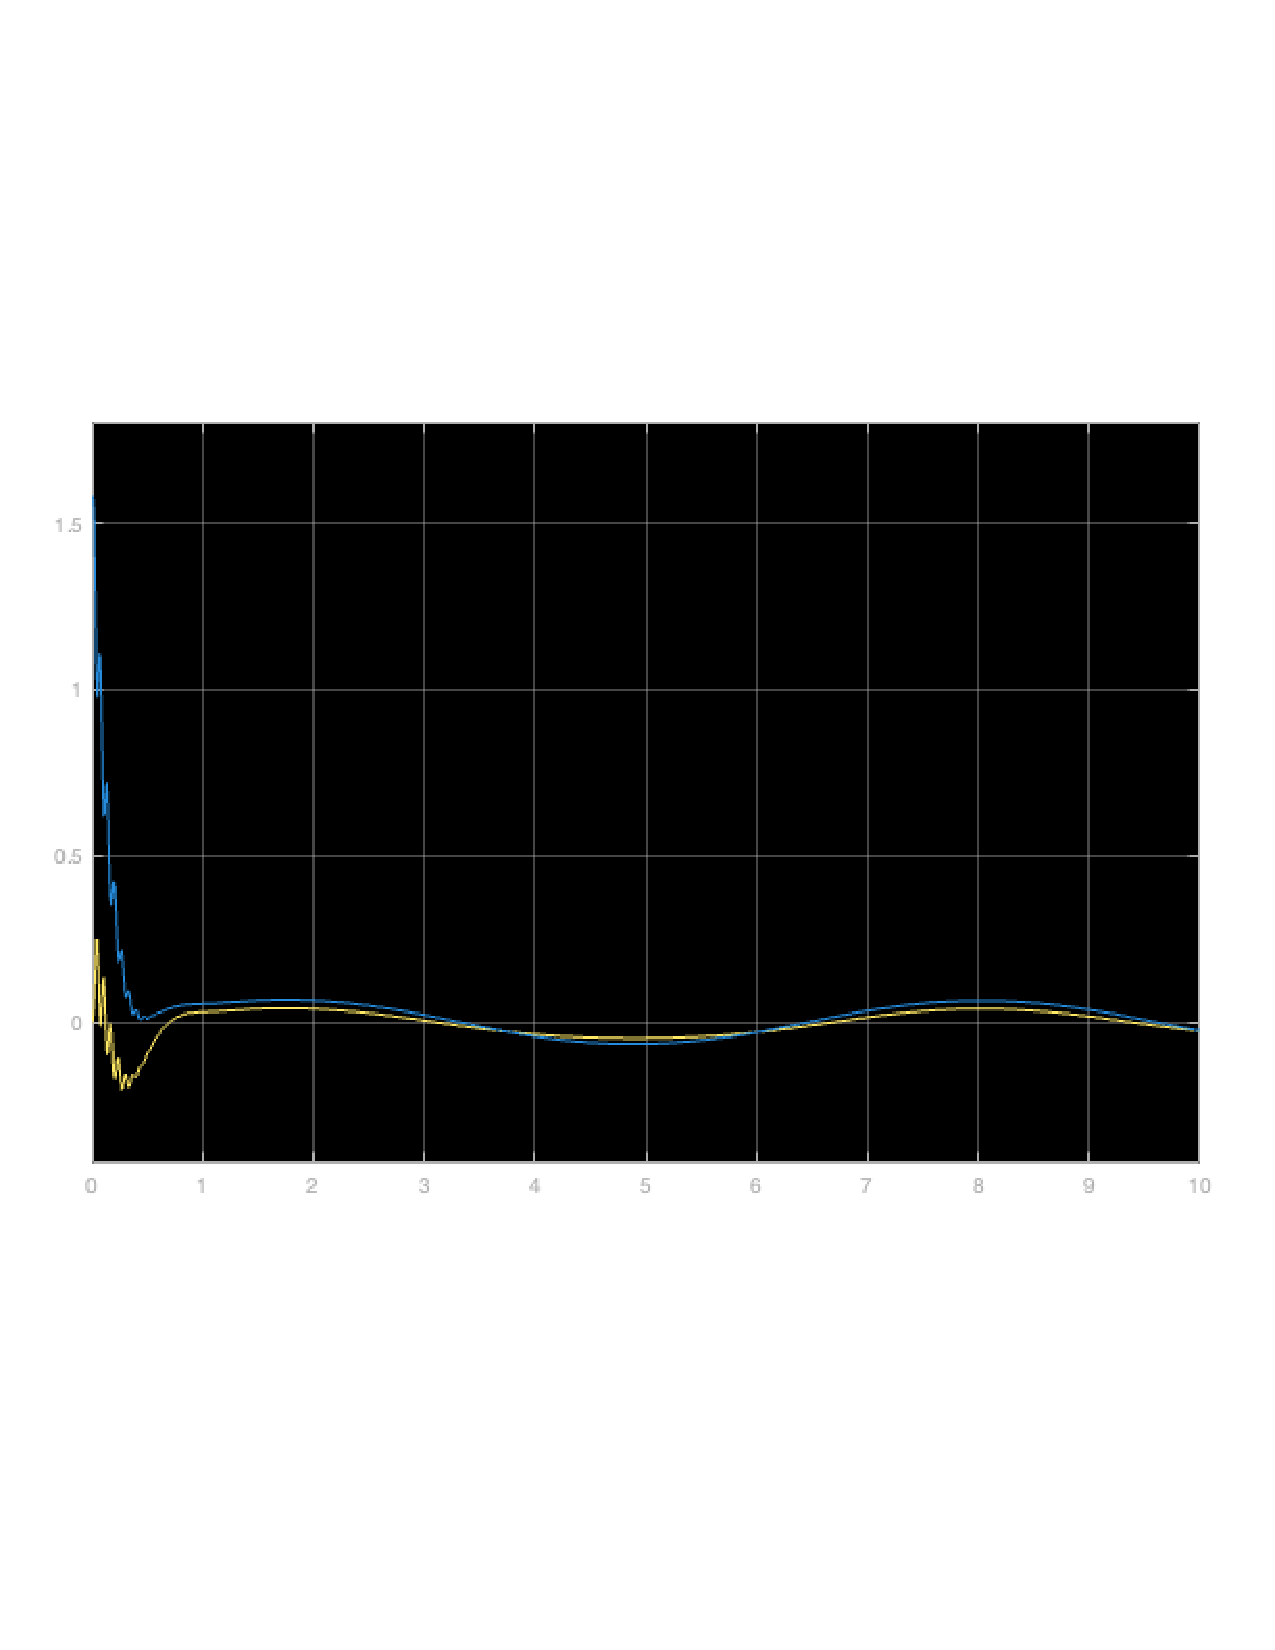
\includegraphics[width=0.8\textwidth]{figures/result_adaptive_controller.pdf}
    \caption{Result Plot, error still exists}
    \label{fig:result_adaptive_controller}
\end{figure}

\newpage

\section{Explanation}

I will try to explain all problems I met and the result I got.\\


\subsection{Computed torques controller}
This part is the same with the part in the last report.\\ 

Pros: 
1. Easy to calculate and understand the process of controlling.\\
2. Allow you fine-tuning the parameters to get better results.\\

Cons:
1. Require robot model parameters, including all lengths and mass.\\
2. If the parameters are not right, easy to make the system not stable.\\

\subsection{Desired task space controller}
The main work of this part is a inverse kinematics block, I choose to directly calculate the angles.\\
There is a shake during controlling, I guess that's because the calculated angle has a big change, there always two results for calculation.\\


\subsection{adaptive controller}
I use the data store memory to store the $\hat{M}$, I need to keep it can be updated all the time.\\

I wonder if there is any other ways to achieve adaptive law.\\

The result is not very beautiful, I guess maybe relative to I only estimate the $M$.\\ 


\end{document}